\subsection{Tableaux multidimensionnels}

En interne, un tableau multidimensionnel est pratiquement la même chose qu'un tableau
linéaire.

Puisque la mémoire d'un ordinateur est linéaire, c'est un tableau uni-dimensionnel.
Par commodité, ce tableau multidimensionnel peut facilement être représenté comme
un uni-dimensionnel.

Par exemple, voici comment les éléments du tableau 3*4 sont placés dans un tableau
uni-dimensionnel de 12 éléments:

% TODO FIXME not clear. First, horizontal would be better. Second, why two columns?
% I'd first show 3x4 with numbered elements (e.g. 32-bit ints) in colored lines,
% then linear with the same numbered elements (and colored blocks)
% then linear with addresses (offsets) - assuming let say 32-bit ints.
\begin{table}[H]
\centering
\begin{tabular}{ | l | l | }
\hline
Offset en mémoire & élément du tableau \\
\hline
0 & [0][0] \\
\hline
1 & [0][1] \\
\hline
2 & [0][2] \\
\hline
3 & [0][3] \\
\hline
4 & [1][0] \\
\hline
5 & [1][1] \\
\hline
6 & [1][2] \\
\hline
7 & [1][3] \\
\hline
8 & [2][0] \\
\hline
9 & [2][1] \\
\hline
10 & [2][2] \\
\hline
11 & [2][3] \\
\hline
\end{tabular}
\caption{Tableau en deux dimensions représenté en mémoire en une dimension}
\end{table}

Voici comment chacun des éléments du tableau 3*4 sont placés en mémoire:

% TODO coordinates. TikZ?
\begin{table}[H]
\centering
\begin{tabular}{ | l | l | l | l | }
\hline                        
0 & 1 & 2 & 3 \\
\hline  
4 & 5 & 6 & 7 \\
\hline  
8 & 9 & 10 & 11 \\
\hline  
\end{tabular}
\caption{Adresse mémoire de chaque élément d'un tableau à deux dimensions}
\end{table}

\myindex{row-major order}

Donc, afin de calculer l'adresse de l'élément voulu, nous devons d'abord multiplier
le premier index par 4 (largeur du tableau) et puis ajouter le second index.
Ceci est appelé \emph{row-major order} (ordre ligne d'abord),
et c'est la méthode de représentation des tableaux et des matrices au moins en \CCpp
et Python.
Le terme \emph{row-major order} est de l'anglais signifiant: \q{ d'abord, écrire les
éléments de la première ligne, puis ceux de la seconde ligne \dots et enfin les éléments
de la dernière ligne}.

\myindex{column-major order}
\myindex{Fortran}
Une autre méthode de représentation est appelée \emph{column-major order} (ordre colonne
d'abord) (les indices du tableau sont utilisés dans l'ordre inverse) et est utilisé
au moins en ForTran, MATLAB et R.
Le terme \emph{column-major order} est de l'anglais signifiant: \q{ d'abord, écrire les
éléments de la première colonne, puis ceux de la seconde colonne \dots et enfin les
éléments de la dernière colonne}.

Quelle méthode est la meilleure?

En général, en termes de performance et de mémoire cache, le meilleur schéma pour
l'organisation des données est celui dans lequel les éléments sont accédés séquentiellement.

Donc si votre fonction accède les données par ligne, \emph{row-major order} est meilleur,
et vice-versa.

% subsubsections
\subsubsection{Exemple de tableau à 2 dimensions}

Nous allons travailler avec un tableau de type \Tchar, qui implique que chaque élément
n'a besoin que d'un octet en mémoire.

\myparagraph{Exemple de remplissage d'une ligne}
\myindex{\olly}

Remplissons la seconde ligne avec les valeurs 0..3:

\lstinputlisting[caption=Exemple de remplissage d'une ligne,style=customc]{patterns/13_arrays/5_multidimensional/two1_FR.c}

Les trois lignes sont entourées en rouge.
Nous voyons que la seconde ligne a maintenant les valeurs 0, 1, 2 et 3:

\begin{figure}[H]
\centering
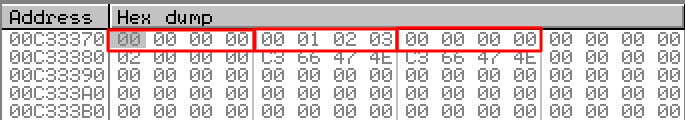
\includegraphics[width=0.6\textwidth]{patterns/13_arrays/5_multidimensional/olly_2D_1.png}
\caption{\olly: le tableau est rempli}
\end{figure}

\myparagraph{Exemple de remplissage d'une colonne}
\myindex{\olly}

Remplissons la troisième colonne avec les valeurs: 0..2:

\lstinputlisting[caption=Exemple de remplissage d'une colonne,style=customc]{patterns/13_arrays/5_multidimensional/two2_FR.c}

Les trois lignes sont entourées en rouge ici.

Nous voyons que dans chaque ligne, à la troisième position, ces valeurs sont écrites:
0, 1 et 2.

\begin{figure}[H]
\centering
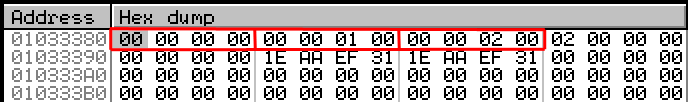
\includegraphics[width=0.6\textwidth]{patterns/13_arrays/5_multidimensional/olly_2D_2.png}
\caption{\olly: le tableau est rempli}
\end{figure}


\subsubsection{Accéder à un tableau en deux dimensions comme un à une dimension}

Nous pouvons facilement nous assurer qu'il est possible d'accéder à un tableau en
deux dimensions d'au moins deux façons:

\lstinputlisting[style=customc]{patterns/13_arrays/5_multidimensional/2D_as_1D_FR.c}

Compilons\footnote{Ce programme doit être compilé comme un programme C, pas C++,
sauvegardez-le dans un fichier avecl'extention .c pour le compiler avec MSVC} le et
lançons le: il montre des valeurs correctes.

Ce que MSVC 2013 a généré est fascinant, les trois routines sont les mêmes!

\lstinputlisting[caption=MSVC 2013 \Optimizing x64,style=customasmx86]{patterns/13_arrays/5_multidimensional/2D_as_1D_MSVC_2013_Ox_x64_FR.asm}

GCC génère des routines équivalentes, mais légèrement différentes:

\lstinputlisting[caption=GCC 4.9 x64 \Optimizing,style=customasmx86]{patterns/13_arrays/5_multidimensional/2D_as_1D_GCC49_x64_O3_FR.s}


\subsubsection{Exemple de tableau à trois dimensions}

C'est la même chose pour des tableaux multidimensionnels.

Nous allons travailler avec des tableaux de type \Tint: chaque élément nécessite
4 octets en mémoire.

Voyons ceci:

\lstinputlisting[caption=simple exemple,style=customc]{patterns/13_arrays/5_multidimensional/multi.c}

\myparagraph{x86}

Nous obtenons (MSVC 2010):

\lstinputlisting[caption=MSVC 2010,style=customasmx86]{patterns/13_arrays/5_multidimensional/multi_msvc_FR.asm}

Rien de particulier. Pour le calcul de l'index, trois arguments en entrée sont utilisés
dans la formule $address=600 \cdot 4 \cdot x + 30 \cdot 4 \cdot y + 4z$, pour représenter
le tableau comme multidimensionnel.
N'oubliez pas que le type \Tint est 32-bit (4 octets), donc tous les coefficients
doivent être multipliés par 4.

\lstinputlisting[caption=GCC 4.4.1,style=customasmx86]{patterns/13_arrays/5_multidimensional/multi_gcc_FR.asm}

Le compilateur GCC fait cela différemment.

Pour une des opérations du calcul ($30y$), GCC produit un code sans instruction de
multiplication. Voici comment il fait:
$(y+y) \ll 4 - (y+y) = (2y) \ll 4 - 2y = 2 \cdot 16 \cdot y - 2y = 32y - 2y = 30y$. 
Ainsi, pour le calcul de $30y$, seulement une addition, un décalage de bit et une
soustraction sont utilisés.
Ceci fonctionne plus vite.

\myparagraph{ARM + \NonOptimizingXcodeIV (\ThumbMode)}

\lstinputlisting[caption=\NonOptimizingXcodeIV (\ThumbMode),style=customasmARM]{patterns/13_arrays/5_multidimensional/multi_Xcode_thumb_O0_FR.asm}

LLVM \NonOptimizing sauve toutes les variables dans la pile locale, ce qui est redondant.

L'adresse de l'élément du tableau est calculée par la formule vue précédemment.

\myparagraph{ARM + \OptimizingXcodeIV (\ThumbMode)}

\lstinputlisting[caption=\OptimizingXcodeIV (\ThumbMode),style=customasmARM]{patterns/13_arrays/5_multidimensional/multi_Xcode_thumb_O3_FR.asm}

L'astuce de remplacer la multiplication par des décalage, addition et soustraction
que nous avons déjà vue est aussi utilisée ici.

\myindex{ARM!\Instructions!RSB}
\myindex{ARM!\Instructions!SUB}
Ici, nous voyons aussi une nouvelle instruction: \RSB (\emph{Reverse Subtract}).

Elle fonctionne comme \SUB, mais échange ses opérandes l'un avec l'autre avant l'exécution.
Pourquoi?
\myindex{ARM!Optional operators!LSL}
\SUB et \RSB sont des instructions auxquelles un coefficient de décalage peut être
appliqué au second opérande: (\INS{LSL\#4}).

Mais ce coefficient ne peut être appliqué qu'au second opérande.

C'est bien pour des opérations commutatives comme l'addition ou la multiplication
(les opérandes peuvent être échangés sans changer le résultat).

Mais la soustraction est une opération non commutative, donc \RSB existe pour ces
cas.

\myparagraph{MIPS}

\myindex{MIPS!Global Pointer}
Mon exemple est minuscule, donc le compilateur GCC a décidé de mettre le tableau
$a$ dans la zone de 64KiB adressable par le Global Pointer.

\lstinputlisting[caption=GCC 4.4.5 \Optimizing (IDA),style=customasmMIPS]{patterns/13_arrays/5_multidimensional/multi_MIPS_O3_IDA_FR.lst}


\subsubsection{Obtenir la dimension d'un tableau multidimensionnel}
\myindex{Hex-Rays}

Toute fonction de traitement de chaîne, à laquelle un tableau de caractère lui est passée,
ne peut pas en déduire la taille de ce tableau en entrée.

Par exemple:

\lstinputlisting[style=customc]{patterns/13_arrays/5_multidimensional/dimensions2.c}

\dots si compilé (par n'importe quel compilateur) et ensuite décompilé par Hex-Rays:

\lstinputlisting[style=customc]{patterns/13_arrays/5_multidimensional/dimensions2_hexrays.c}

Il n'y a pas moyen de trouver la taille de la première dimension.
Si la valeur $x$ passée est trop grosse, un dépassement de tampon peut se produire,
un élément d'un endroit aléatoire en mémoire sera lu.

Et un tableau 3D:

\lstinputlisting[style=customc]{patterns/13_arrays/5_multidimensional/dimensions3.c}

Hex-Rays:

\lstinputlisting[style=customc]{patterns/13_arrays/5_multidimensional/dimensions3_hexrays.c}

À nouveau, seules deux des 3 dimensions peuvent être déduites.


\subsubsection{Plus d'exemples}

L'écran de l'ordinateur est représenté comme un tableau 2D, mais le buffer vidéo
est un tableau linéaire 1D.
Nous en parlons ici: \myref{Mandelbrot_demo}.

Un autre exemple dans ce livre est le jeu Minesweeper: son champ est aussi un tableau
à deux dimensions: \myref{minesweeper_winxp}.

